\section{Open data sources}

The analysis carried out will utilise the Greater London area as the working case study, serving as an example for further replications of the analysis for other localities. The Office for National Statistics (ONS) defines the Greater London metropolitan area to include the City of London and the 32 London boroughs, with a total area of 1,572 km$^2$ and a population of 9.4 million people, making it the largest in the United Kingdom. The choice of the Greater London metropolitan area is also motivated by the availability of open data sources from which necessary features could be derived and the complexity of the public transport network, coupled with rich usage data made available to the public. The data sources used in this analysis are summarised in Table \ref{tab:datasources} and detailed below.

\begin{table}[ht]
    \centering
    \renewcommand{\arraystretch}{1.5}
    \begin{tabular}{|l|l|l|}
        \hline 
        \rowcolor{lightgray}
        \textbf{} & \textbf{Variables} & \textbf{Sources} \\
        \hline

        \multirow{2}{12em}{\textbf{Public transport arrivals (target)}} 
        & Tube and Rail station exits & TfL network demand (NUMBAT) \\ 
        & Bus alightings & TfL network demand (BUSTO) \\
        \hline

        \textbf{Population} & Population count & UK Census 2021 \\
        \hline

        \multirow{2}{12em}{\textbf{Amenity Profile}} 
        & POI count by type & OSM Amenity POIs \\ 
        & POI diversity index & \\ 
        \hline 

        \multirow{3}{12em}{\textbf{Public Transport (PT) Connectivity Profile}} 
        & PT node count by type &  \\
        & PT node diversity index & OSM Transport POIs and TfL \\
        & PT network centrality &  \\
        \hline

            \end{tabular}
    \caption{Summary of data used in the analysis and their sources}
    \label{tab:datasources}
\end{table}

\subsubsection*{Transport for London (TfL) Open Data}

We use the following GIS datasets from the \href{https://gis-tfl.opendata.arcgis.com/}{TfL GIS Open Data Hub} and \href{https://api.tfl.gov.uk/}{TfL API} to derive transport-related features for the study area including density of transport facilities, diversity of transport options, and accessibility in the form of centrality measures in the Rail and Bus networks separately. The networks of interest are defined as follows:

\begin{itemize}
    \setlength\itemsep{0em}
    \item \textit{Rail network} includes the London Underground, London Overground, the Docklands Light Railway, and the Elizabeth Line, excluding stations and segments that are not managed by TfL or fall outside the Greater London area.
    \item \textit{Bus network} includes stop locations and route data of all bus and tram services, excluding stops and route segments that are not managed by TfL or within the Greater London area.
\end{itemize}

TfL also provides annually-updated \href{http://crowding.data.tfl.gov.uk/}{network demand datasets}, which will be used to derive the target variables of our analysis. The datasets of special interest to our analysis are namely \textit{Rail demand data (NUMBAT)} and the \textit{Bus demand data (BUSTO)}, from which we will extract estimated counts of station exits and bus alightings at the station or stop level, respectively. The dataset's temporal granularity is also an important aspect to consider. To address non-commute trips for the analysis, we will specifically use \textbf{average Saturday demand}, representing the demand in a typical period without any major citywide disruptions or events\footnote{This Saturday travel demand may still include work trips for those working on Saturdays, albeit not concentrated into peak periods as with weekday travel demand. For the scope of this analysis, we will treat these potential work trips as non-commute.}. To examine possible variations between different times of day, besides the total counts of exits and bus alightings in one day, we will aggregate the data into four larger time bands\footnote{The choice of time band delineation is a compromise between different granularity levels afforded by the TfL rail and the bus demand datasets. There are opportunities to deepen the analysis by further segmenting the time bands into finer intervals if data permits.}:

\begin{itemize}
    \setlength\itemsep{-0.2em}
    \item \textit{Morning} (05:00 - 10:00): Limited mobility expected due to early hours
    \item \textit{Midday} (10:00 - 19:00): High daytime mobility expected
    \item \textit{Evening} (19:00 - 00:00): High evening mobility expected
    \item \textit{Late} (00:00 - 05:00): Minimal mobility expected due to sparser night PT services
\end{itemize}

It is worth noting that despite the existence of the Oyster Card integrated fare system, TfL does not provide origin-destination data as open data. Therefore, station exits and bus alightings are not directly associated with the number of passengers traversing through the system but are treated as discrete events. For example, a person who takes a bus to reach a Tube station for onward travel and then exits to arrive at their destination would be counted as two separate data points, one alighting for the bus and one station exit for the Tube. Nevertheless, our model will take this into account when making porediction and allows us to investigate patterns and the contribution of modal interchange behaviour in our interpretation.

Lastly, we need to acknowledge the particularity of the TfL bus demand dataset (BUSTO). Although passengers do not 'tap off' when alighting from busses, TfL has adopted a methodology to estimate the number of passengers alighting at each bus stop based on individuals' next actions and other statistical methods. The methodology is described in the \href{http://crowding.data.tfl.gov.uk/BUSTO/BUSTO\%20User\%20Guide\%20and\%20Data\%20Dictionary\%20v1.0.pdf}{BUSTO User Guide and Data Dictionary}

\subsubsection*{UK Census Data 2021}
For the estimated population datasets, we rely on the most recent United Kingdom Census data administered in 2021. The data is ingested at the Output Area (OA) level, which is the smallest geographical unit for which census data is available. Further processing will aggregate the data to the desired spatial unit of analysis.

\subsubsection*{OpenStreetMap POIs}
OpenStreetMap (OSM) is a collaborative mapping project that provides a free and open-source map of the world. The version of OSM data used in this analysis is packaged by an OpenStreetMap community project \href{https://www.geofabrik.de/en/geofabrik/openstreetmap.html}{Geofabrik} and provides a snapshot of the OSM database as of June 2024. Geofabrik also standardises the categorisation of POIs' amenity attributes in the OSM database into larger classes\footnote{More information about Geofabrik's OSM data product can be found in \href{https://www.geofabrik.de/data/geofabrik-osm-gis-standard-0.6.pdf}{Geofabrik OSM data dictionary}}. Our analysis will use this default POI classification, extracting 12 amenity POI types. Lastly, apart from amenity POIs, we also make use of the OSM transport POIs point data to derive non-TfL transport-related features, such as national rail stations, ferry piers, long-distance bus stations and airports. 

Combined with transport node data acquired from TfL open data sources, all extracted Amenity and Transport POI types of interest are summarised in Table \ref{tab:osmpoi}.

\begin{table}[ht]
    \centering
    \renewcommand{\arraystretch}{1.1}
    \begin{tabular}{|l|l|l|}
        \hline
        \rowcolor{lightgray}
        & \textbf{POI Type} & \textbf{Examples} \\
        \hline
        \multirow{13}{*}{\textbf{Amenity}}
            &\textit{Public Facilities} & Post offices, schools, universities, libraries,... \\
            &\textit{Medical} & Hospitals, clinics, pharmacies,... \\
            &\textit{Entertainment} & Theatres, Night clubs, cinemas,... \\
            &\textit{Outdoors} & Parks, playgrounds,... \\
            &\textit{Active} & Sports centres, swimming pools, stadiums,... \\
            &\textit{Restaurants} & Restaurants, cafes, pubs, bars,... \\
            &\textit{Hotels} & Hotels, motels, hostels,... \\
            &\textit{Shopping} & Supermarkets, bakeries, florists, bookshops, malls,... \\
            &\textit{Banking} & Banks, ATMs,... \\
            &\textit{Tourism} & Tourist attractions, museums, monuments, viewpoints,... \\
            &\textit{Religious} & Churches, mosques, temples,... \\
            &\textit{Nature} & Riverbanks, beaches, hills,... \\
        \hline
        \multirow{3}{*}{\textbf{Transport}}
            &\textit{Bus stops} & Bus stops and stations (TfL) \\
            &\textit{Rail stations} & TfL rail stations (TfL) and Non-TfL rail stations (OSM) \\
            &\textit{Other transport hubs} & Airports, ferry piers, long-distance bus stations (OSM) \\
        \hline
    \end{tabular}
    \caption{Summary of Amenity and Transport POI types used in the analysis}
    \label{tab:osmpoi}
\end{table}

% \section{True to Data and True to Model in SHAP technique}

% One ongoing debate regarding the use of SHAP for explainable is captured by \citet{chenTrueModelTrue2020}'s work exploring 'True to Model' versus 'True to Data' explanations. The 'True to Data' approach produces \textit{observational SHAP values} which reflect how a feature contributes to the model's prediction when considering the dependencies and correlations present in the training data, whereas the 'True to Model' approach produces \textit{interventional SHAP values} which reveal how a feature influences the model's prediction if we manipulate it independently, regardless of how it might interact with other features in reality. In our case, as we are more interested in observing feature contribution to the model prediction in a controlled environment rather than observing the relationships between features, we will use the 'True to Model' approach to interpret the model's prediction made possible by the \textit{shap} package. This means SHAP values are calculated by iteratively entering features from a sample dataset into the model and observing the change in prediction, effectively isolating the feature's contribution to the model's prediction rather than explaining the feature contribution using the tree paths alone.

\newpage
\section{Supplemental Figures}
\begin{figure}[ht]
    \centering
    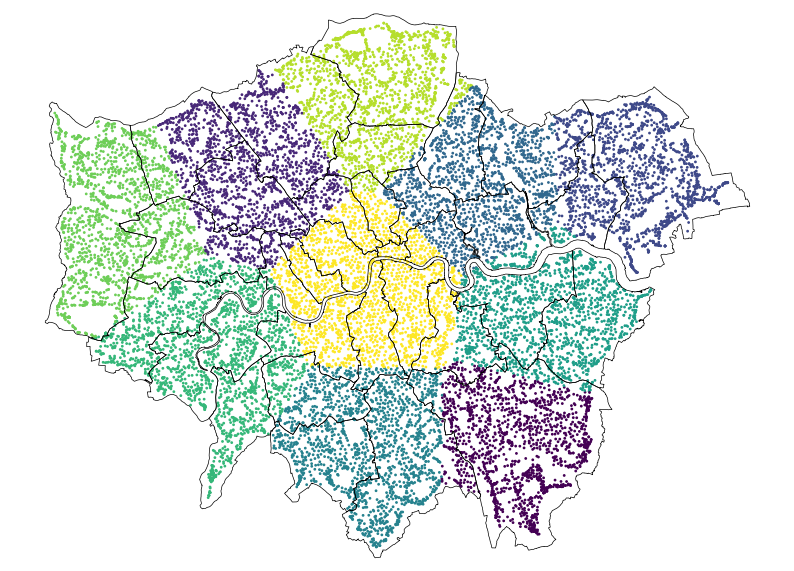
\includegraphics[width=0.5\textwidth]{kfold.png}
    \captionsetup{justification=centering}
    \caption{Map of the spatial k-fold cross-validation splits\\for hyperparameter tuning and performance assessment (k=10)}
    \label{fig:kfold}
\end{figure}

\begin{figure}[!ht]
    \centering
    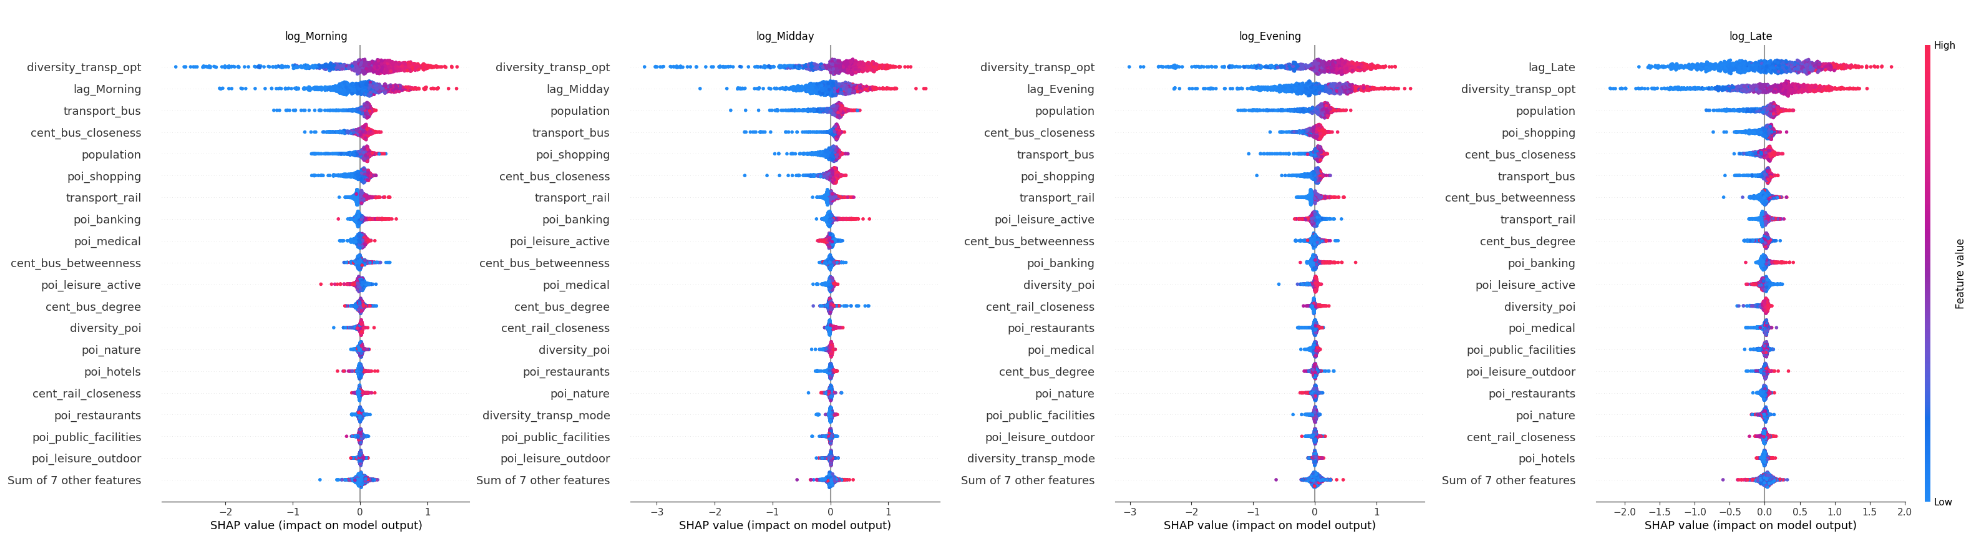
\includegraphics[width=\textwidth]{summarytimeband.png}
    \captionsetup{justification=centering}
    \caption{Summary of feature importance based on SHAP values of a sample. Red-Blue scale represents the feature value, and the x-axis represents the SHAP value, i.e., impact on final model prediction of arrivals in each time band (log)}
    \label{fig:beeswarmtimeband}
\end{figure}